\documentclass[
mode=present,
nohandoutpagebreaks,
nohandoutframes,
size=12pt,
style=huskyinverse,
hlsections,
slidesnotes,
pauseslide,
clock,
]{powerdot}
\usepackage{amsmath}
\usepackage{pifont}
\usepackage{bbding}
\usepackage{graphicx}
\usepackage{multirow}
\usepackage[]{xcolor}
\usepackage{tikz}
\usetikzlibrary{shapes.callouts}
\usepackage[most]{tcolorbox}
\newtcolorbox{mybox}[2][]{colback=red!5!white,
colframe=red!75!black,fonttitle=\bfseries,
colbacktitle=red!85!black,enhanced,
attach boxed title to top center={yshift=-2mm},
title=#2,#1}
\definecolor{mycolor}{HTML}{00F9DE}
\graphicspath{{./figures/}}
\usepackage{array}
% vertically center the text with fixed column width
\newcolumntype{L}[1]{>{\raggedright\let\newline\\\arraybackslash\hspace{0pt}}m{#1}}
\newcolumntype{C}[1]{>{\centering\let\newline\\\arraybackslash\hspace{0pt}}m{#1}}
\newcolumntype{R}[1]{>{\raggedleft\let\newline\\\arraybackslash\hspace{0pt}}m{#1}}

\newcommand{\Dead}{\textcolor{black}{Dead}}
\newcommand{\Hot}{\textcolor{red}{Hot}}
%\usepackage{pdfpages}
\usepackage{fontawesome}
%\usepackage{amsmath}

%\input{tikz_zoom.tex}

%\pddefinetemplate[basic]{slide}{}{\psdots[linecolor=red,dotsize=10pt](0.3\slidewidth,0.5\slideheight)}
\pdsetup{
%palette=green,
%theslide,
%clockformat=h:MM tt,
clockformat=HH:MM:ss,
lf=self-intro,
cf=\today,
rf=mhzhao,
%trans=,
%logohook=tr,
%logopos={0.088\slidewidth,0.99\slideheight},
%logocmd={\includegraphics[height=0.08\slideheight]{}},
%randomdots,
%dprop{dotstyle=ocircle,linewidth=.25pt},
%dmindots=5,dmaxdots=20,
%dminsize=200pt,dmaxsize=700pt,
%dbright=50,
}

\title{\textcolor{magenta}{\faFilePowerpointO}\ Self-instroduction \textcolor{green}{\faAt}SpinFest 2016}
\author{\textcolor{red}{\faCopyright}\textcolor{green}{\faAt}\textcolor{white}{\faUser} Minghui Zhao \\ \\ 
    \textcolor{green}{\faAt}\textcolor{white}{\faUniversity} ISU \ 
    \textcolor{green}{\faAt}\textcolor{white}{\faUniversity} BNL \\
    \rput[lt](-2.10cm,-0.55cm){
\includegraphics[scale=0.40]{dropbox.eps}}
    \rput[lt](-6.5cm,0.75cm){
\includegraphics[scale=0.40]{googledrive.eps}}
    \rput[lt](2.3cm,0.75cm){
\includegraphics[scale=0.40]{onedrive.eps}}
}
\date{\vspace{-0.8cm}\textcolor{white}{\faCalendarCheckO}\ \today}


\begin{document}

\maketitle


\begin{slide}[toc=]{Overview}
\tableofcontents[content=all]
\end{slide}

\section[]{Self-instroduction}
\begin{slide}{self-intro}
%    \rput[lt](-2.8cm,-6.0cm){
\includegraphics[scale=0.050]{Iowa_State_Cyclones.eps}}
    \vspace{-0.3cm}
    \textcolor{red}{\ding{43}}\ I come from Kaifeng,located in east-central China, one of the Eight Ancient Captitals of China.\\
    \vspace{0.1cm}
    \textcolor{green}{\ding{43}}\ Started my Ph.D pursing in Fall, 2014, Iowa State University, superwised under Dr. John Lajoie. Finished courses and passed qualification exams. \\
    \vspace{0.1cm}
    \textcolor{red}{\ding{43}}\ I began with STAR spin group to learn stuffs this summer and I plan to stay in BNL for the next 3 years. \\
    \vspace{0.1cm}
    \textcolor{green}{\ding{43}}\ I will participate in building Postshower detector soon.
    \rput[lt](3.0cm,0.30cm){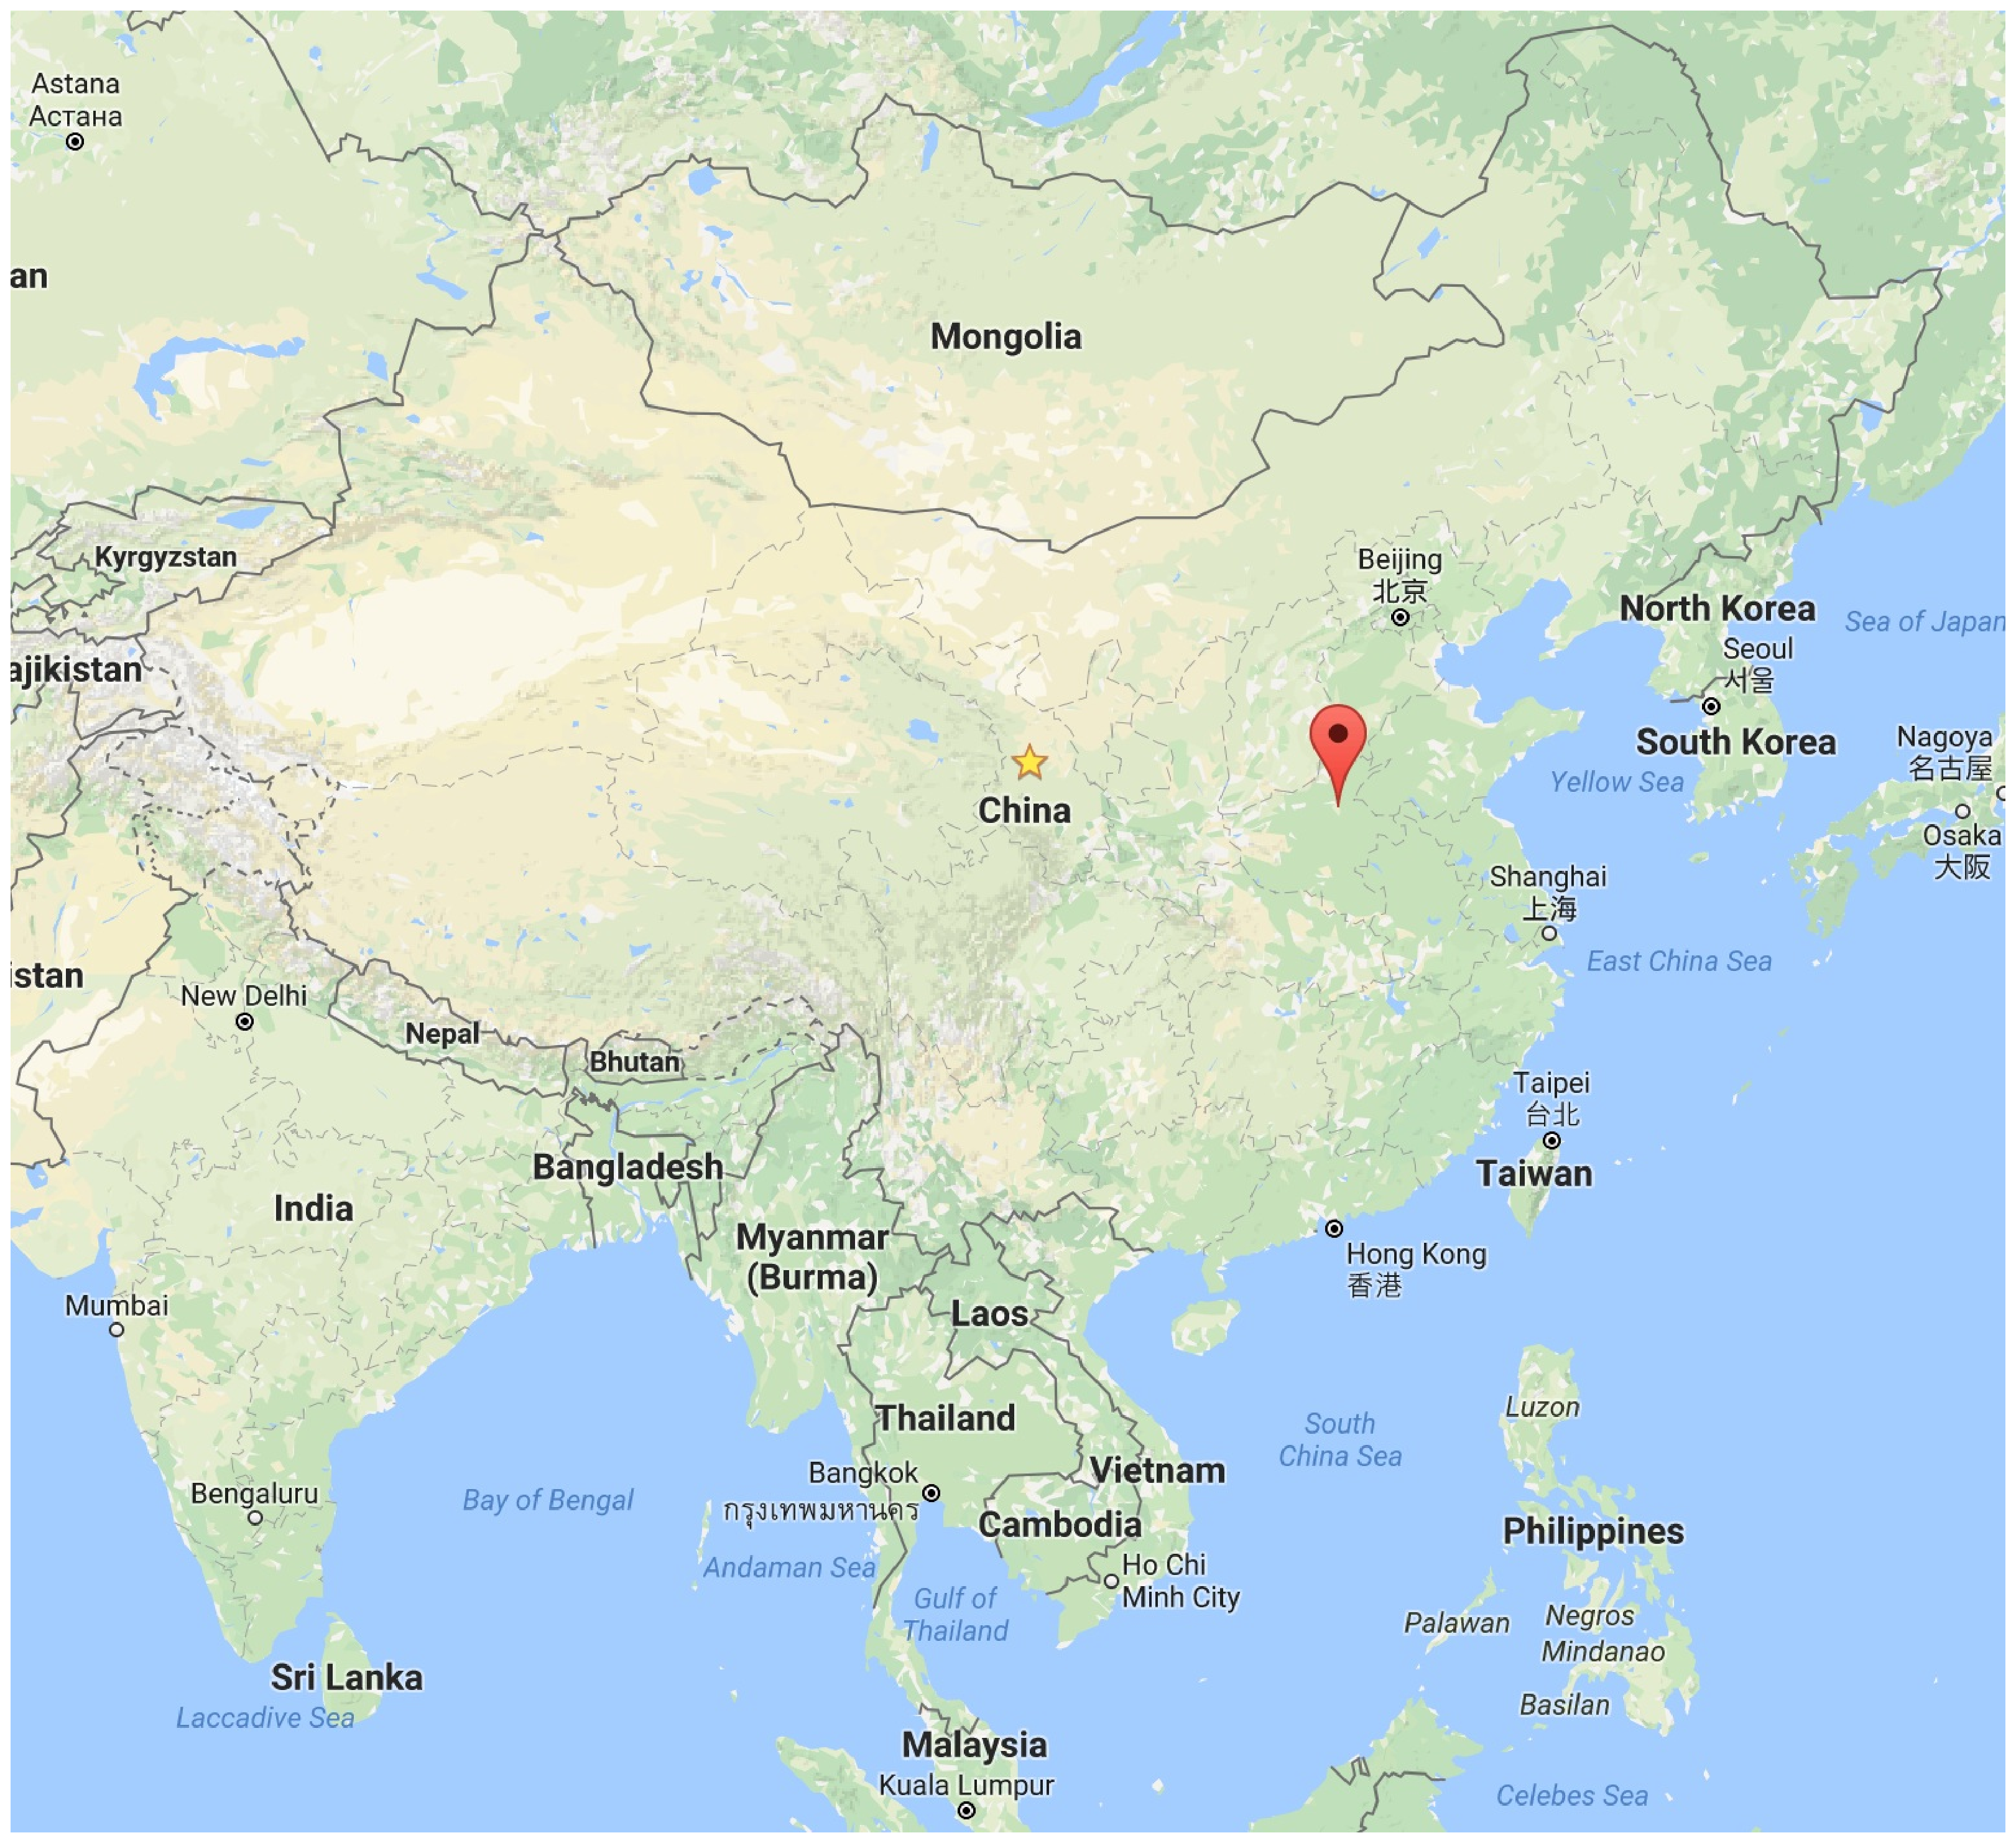
\includegraphics[scale=0.08]{kaifeng.eps}}
\end{slide}

\begin{slide}{Interests}
    \textcolor{red}{\ding{43}}\ Passionate in coding, Linux, Open Source\dots \\
    \vspace{0.5cm}
    \textcolor{green}{\ding{43}}\ Interested in electonics, robotics, 3D printer\dots \\
    \vspace{0.5cm}
    \textcolor{red}{\ding{43}}\ Want to learn more about artificial intellegence, machine learning, big data\dots \\
    \vspace{0.5cm}
    \textcolor{green}{\ding{43}}\ Read tech-news everyday, like watching reviews of new-tech products. \\
    \vspace{0.5cm}
    \textcolor{red}{\ding{43}}\ Call me if you have any software or hardware activities in BNL.
\end{slide}

\section[
%palette=orange,
%template=wideslide,
%tocsection=true,
%slide=true,
%toc=,
%bm=,
]{A little intro my work}

\begin{slide}{FMS Simulation}
    \textcolor{red}{\ding{45}}\ Forward Meson Spectrometer \& Preshower \& Postshower measure $A_N$ of Drell-Yan production($e^{-}/e^{+}$). \\
    \vspace{0.3cm}
    \textcolor{green}{\ding{45}}\ Challenge is to suppress the larger hadron process, which is on the order of $10^5\sim 10^6$ than DY process. \\
    \vspace{0.3cm}
    \textcolor{red}{\ding{43}}\ FMS cut will separate $\mu^{-}$, most part of hadrons. \\
    \vspace{0.3cm}
    \textcolor{green}{\ding{43}}\ plus Preshower first two layers cut will separate $\gamma$ from charged particles. \\
    \vspace{0.3cm}
    \textcolor{red}{\ding{43}}\ plus Preshower third layer cut will separate $e^{-}$ from hadron. \\
    \vspace{0.3cm}
    \textcolor{green}{\ding{43}}\ plus Postshower cut will provide $e^{-}$ separation from hadron improvement. 
\end{slide}
\begin{slide}{Geometry Look}
    \onslide*{1-2}{
        \rput[lt](4cm,0){Overall Look}
    \rput[lt](0.0cm,3.00cm){\includegraphics[scale=0.5]{gamma_overview2.ps}}
    }   
    \onslide*{2}{
    \begin{tikzpicture}[remember picture, overlay]
        \draw[solid] (5.25,-3.6) circle (2.5);
        \path [draw=none,fill=gray, fill opacity =0.2] (5.25, -3.6) circle (2.5);
        \draw (8.7,-4.5) rectangle (8.95,-2.5);
        \path [draw=none,fill=gray, fill opacity =0.2] (8.7, -4.5) rectangle (8.95,-2.5);
        \draw (8.95,-4.5) rectangle (9.4,-2.5);
        \path [draw=none,fill=red, fill opacity =0.2] (8.95, -4.5) rectangle (9.4,-2.5);
        \draw (9.50,-4.5) rectangle (9.7,-2.5);
        \path [draw=none,fill=gray, fill opacity =0.2] (9.50, -4.5) rectangle (9.7,-2.5);
    \end{tikzpicture}
    \begin{tikzpicture}[remember picture, note/.style={rectangle callout, fill=#1},overlay]
        \node [note=red!70,callout relative pointer={(0,1)}] at (5.2,-7.6) {STAR};
        \node [note=red!70,callout relative pointer={(0,-1)}] at (9.1,-1.5) {FMS};
        \node [note=red!70,callout relative pointer={(0,1.5)}] at (9.5,-6.1) {Postshower};
        \node [note=red!70,callout relative pointer={(0,0.7)}] at (8.7,-5.4) {Preshower};
    \end{tikzpicture}
    }
    \onslide*{3}{
        \rput[lt](4cm,0){Close Look}
    \rput[lt](0.0cm,3.50cm){\includegraphics[scale=0.5]{gamma_closelook.ps}}
    }
\end{slide}
\begin{wideslide}{How it works}
    \onslide*{1}{
    
\begin{tikzpicture}[remember picture, overlay]
        \draw[solid] (0.00,-0.2) circle (0.1) (2.40,-0.2) circle (0.1) (4.80,-0.2) circle (0.1);
        \path [draw=none,fill=green, fill opacity =1.0] (0.00, -0.2) circle (0.1);
        \path [draw=none,fill=red, fill opacity =1.0] (2.40, -0.2) circle (0.1);
        \path [draw=none,fill=blue, fill opacity =1.0] (4.80, -0.2) circle (0.1);
        %gamma pre layer 1
        \draw[solid] (2.50,-2.5) circle (0.027);
        \path [draw=none,fill=green, fill opacity =1.0] (2.50, -2.5) circle (0.027);
        %gamma pre layer 2
        \draw[solid] (4.00,-2.5) circle (0.033);
        \path [draw=none,fill=green, fill opacity =1.0] (4.00, -2.5) circle (0.033);
        %gamma pre layer 3
        \draw[solid] (5.40,-2.5) circle (0.100) (5.60,-2.5) circle (0.100) (5.80,-2.5) circle (0.100) (5.40,-2.7) circle (0.100) (5.60,-2.7) circle (0.100) (5.80,-2.7) circle (0.100) (6.00,-2.7) circle (0.032);
        \path [draw=none,fill=green, fill opacity =1.0] (5.40, -2.5) circle (0.100) (5.60, -2.5) circle (0.100) (5.80, -2.5) circle (0.100) (5.40, -2.7) circle (0.100) (5.60, -2.7) circle (0.100) (5.80, -2.7) circle (0.100) (6.00, -2.7) circle (0.032);
        %gamma FMS
        \draw[solid] (6.80,-2.4) circle (0.100);
        \path [draw=none,fill=red, fill opacity =1.0] (6.80, -2.4) circle (0.100);
        \draw[solid] (7.00,-2.4) circle (0.100);
        \path [draw=none,fill=red, fill opacity =1.0] (7.00, -2.4) circle (0.100);
        \draw[solid] (7.20,-2.4) circle (0.100);
        \path [draw=none,fill=red, fill opacity =1.0] (7.20, -2.4) circle (0.100);
        \draw[solid] (7.40,-2.4) circle (0.100);
        \path [draw=none,fill=red, fill opacity =1.0] (7.40, -2.4) circle (0.100);
        \draw[solid] (6.80,-2.6) circle (0.100);
        \path [draw=none,fill=red, fill opacity =1.0] (6.80, -2.6) circle (0.100);
        \draw[solid] (7.00,-2.6) circle (0.100);
        \path [draw=none,fill=red, fill opacity =1.0] (7.00, -2.6) circle (0.100);
        \draw[solid] (7.20,-2.6) circle (0.100);
        \path [draw=none,fill=red, fill opacity =1.0] (7.20, -2.6) circle (0.100);
        \draw[solid] (7.40,-2.6) circle (0.100);
        \path [draw=none,fill=red, fill opacity =1.0] (7.40, -2.6) circle (0.100);
        \draw[solid] (6.80,-2.8) circle (0.100);
        \path [draw=none,fill=red, fill opacity =1.0] (6.80, -2.8) circle (0.100);
        \draw[solid] (7.00,-2.8) circle (0.100);
        \path [draw=none,fill=red, fill opacity =1.0] (7.00, -2.8) circle (0.100);
        \draw[solid] (7.20,-2.8) circle (0.100);
        \path [draw=none,fill=red, fill opacity =1.0] (7.20, -2.8) circle (0.100);
        \draw[solid] (7.40,-2.8) circle (0.100);
        \path [draw=none,fill=red, fill opacity =1.0] (7.40, -2.8) circle (0.100);
        \draw[solid] (6.80,-3.0) circle (0.100);
        \path [draw=none,fill=red, fill opacity =1.0] (6.80, -3.0) circle (0.100);
        \draw[solid] (7.00,-3.0) circle (0.078);
        \path [draw=none,fill=red, fill opacity =1.0] (7.00, -3.0) circle (0.078);
        %gamma post layer 1
        \draw[solid] (8.30,-2.5) circle (0.100) (8.50,-2.5) circle (0.076);
        \path [draw=none,fill=blue, fill opacity =1.0] (8.30,-2.5) circle (0.100) (8.50,-2.5) circle (0.076);
        %gamma post layer 2
        \draw[solid] (9.80,-2.5) circle (0.100) (10.00,-2.5) circle (0.064);
        \path [draw=none,fill=blue, fill opacity =1.0] (9.80,-2.5) circle (0.100) (10.00,-2.5) circle (0.064);
        %gamma post layer 3
        \draw[solid] (11.80,-2.5) circle (0.100) (12.00,-2.5) circle (0.034);
        \path [draw=none,fill=blue, fill opacity =1.0] (11.80,-2.5) circle (0.100) (12.00,-2.5) circle (0.034);
        %electron pre layer 1
        \draw[solid] (2.50,-3.5) circle (0.100) (2.70,-3.5) circle (0.023);
        \path [draw=none,fill=green, fill opacity =1.0] (2.50,-3.5) circle (0.100) (2.70,-3.5) circle (0.023);
        %electron pre layer 2
        \draw[solid] (4.00,-3.5) circle (0.100) (4.20,-3.5) circle (0.034);
        \path [draw=none,fill=green, fill opacity =1.0] (4.00,-3.5) circle (0.100) (4.20,-3.5) circle (0.034);
        %electron pre layer 3
        \draw[solid] (5.40,-3.4) circle (0.100) (5.60,-3.4) circle (0.1) (5.80,-3.4) circle (0.1) (6.00,-3.4) circle (0.1) (5.40,-3.6) circle (0.100) (5.60,-3.6) circle (0.1) (5.80,-3.6) circle (0.1) (6.00,-3.6) circle (0.1) (5.40,-3.8) circle (0.100) (5.60,-3.8) circle (0.1) (5.80,-3.8) circle (0.1) (6.00,-3.8) circle (0.100) (5.40,-4.0) circle (0.053);
        \path [draw=none,fill=green, fill opacity =1.0] (5.40,-3.4) circle (0.100) (5.60,-3.4) circle (0.1) (5.80,-3.4) circle (0.1) (6.00,-3.4) circle (0.1) (5.40,-3.6) circle (0.100) (5.60,-3.6) circle (0.1) (5.80,-3.6) circle (0.1) (6.00,-3.6) circle (0.1) (5.40,-3.8) circle (0.100) (5.60,-3.8) circle (0.1) (5.80,-3.8) circle (0.1) (6.00,-3.8) circle (0.100) (5.40,-4.0) circle (0.053);
        %electron FMS
        \draw[solid] (6.80,-3.4) circle (0.100) (7.00,-3.4) circle (0.100) (7.20,-3.4) circle (0.100) (7.40,-3.4) circle (0.100) (6.80,-3.6) circle (0.100) (7.00,-3.6) circle (0.100) (7.20,-3.6) circle (0.100) (7.40,-3.6) circle (0.100) (6.80,-3.8) circle (0.100) (7.00,-3.8) circle (0.100) (7.20,-3.8) circle (0.100) (7.40,-3.8) circle (0.100) (6.80, -4.0) circle (0.100) (7.00, -4.0) circle (0.073);
        \path [draw=none,fill=red, fill opacity =1.0] (6.80,-3.4) circle (0.100) (7.00,-3.4) circle (0.100) (7.20,-3.4) circle (0.100) (7.40,-3.4) circle (0.100) (6.80,-3.6) circle (0.100) (7.00,-3.6) circle (0.100) (7.20,-3.6) circle (0.100) (7.40,-3.6) circle (0.100) (6.80,-3.8) circle (0.100) (7.00,-3.8) circle (0.100) (7.20,-3.8) circle (0.100) (7.40,-3.8) circle (0.100) (6.80, -4.0) circle (0.100) (7.00, -4.0) circle (0.073);
        %electron post layer 1
        \draw[solid] (8.30,-3.5) circle (0.100) (8.50,-3.5) circle (0.017);
        \path [draw=none,fill=blue, fill opacity =1.0] (8.30,-3.5) circle (0.100) (8.50,-3.5) circle (0.017);
        %electron post layer 2
        \draw[solid] (9.80,-3.5) circle (0.100) (10.00,-3.5) circle (0.009);
        \path [draw=none,fill=blue, fill opacity =1.0] (9.80,-3.5) circle (0.100) (10.00,-3.5) circle (0.009);
        %electron post layer 3
        \draw[solid] (11.80,-3.5) circle (0.089);
        \path [draw=none,fill=blue, fill opacity =1.0] (11.80,-3.5) circle (0.089);
        %pi- pre layer 1
        \draw[solid] (2.50,-4.5) circle (0.100) (2.70,-4.5) circle (0.094);
        \path [draw=none,fill=green, fill opacity =1.0] (2.50,-4.5) circle (0.100) (2.70,-4.5) circle (0.094);
        %pi- pre layer 2
        \draw[solid] (4.00,-4.5) circle (0.100) (4.20,-4.5) circle (0.100) (4.40,-4.5) circle (0.0344);
        \path [draw=none,fill=green, fill opacity =1.0] (4.00,-4.5) circle (0.100) (4.20,-4.5) circle (0.100) (4.40,-4.5) circle (0.0344);
        %pi- pre layer 3
        \draw[solid] (5.40,-4.5) circle (0.100) (5.60,-4.5) circle (0.100) (5.80,-4.5) circle (0.100) (6.00,-4.5) circle (0.100) (5.40,-4.7) circle (0.055);
        \path [draw=none,fill=green, fill opacity =1.0] (5.40,-4.5) circle (0.100) (5.60,-4.5) circle (0.100) (5.80,-4.5) circle (0.100) (6.00,-4.5) circle (0.100) (5.40,-4.7) circle (0.055);
        %pi- FMS
        \draw[solid] (6.80,-4.5) circle (0.100) (7.00,-4.5) circle (0.100) (7.20,-4.5) circle (0.100) (7.40,-4.5) circle (0.100) (6.80,-4.7) circle (0.024);
        \path [draw=none,fill=red, fill opacity =1.0] (6.80,-4.5) circle (0.100) (7.00,-4.5) circle (0.100) (7.20,-4.5) circle (0.100) (7.40,-4.5) circle (0.100) (6.80,-4.7) circle (0.024);
        %pi- post layer 1
        \draw[solid] (8.30,-4.5) circle (0.100) (8.50,-4.5) circle (0.10) (8.70,-4.5) circle (0.10) (8.90,-4.5) circle (0.100) (8.30,-4.7) circle (0.100) (8.50,-4.7) circle (0.10) (8.70,-4.7) circle (0.10) (8.90,-4.7) circle (0.100) (8.30,-4.9) circle (0.068);
        \path [draw=none,fill=blue, fill opacity =1.0] (8.30,-4.5) circle (0.100) (8.50,-4.5) circle (0.10) (8.70,-4.5) circle (0.10) (8.90,-4.5) circle (0.100) (8.30,-4.7) circle (0.100) (8.50,-4.7) circle (0.10) (8.70,-4.7) circle (0.10) (8.90,-4.7) circle (0.100) (8.30,-4.9) circle (0.068);
        %pi- post layer 2
        \draw[solid] (9.80,-4.5) circle (0.100) (10.00,-4.5) circle (0.100) (10.20,-4.5) circle (0.100) (10.40,-4.5) circle (0.10) (9.80,-4.7) circle (0.100) (10.00,-4.7) circle (0.100) (10.20,-4.7) circle (0.100) (10.40,-4.7) circle (0.10) (9.80,-4.9) circle (0.073);
        \path [draw=none,fill=blue, fill opacity =1.0] (9.80,-4.5) circle (0.100) (10.00,-4.5) circle (0.100) (10.20,-4.5) circle (0.100) (10.40,-4.5) circle (0.10) (9.80,-4.7) circle (0.100) (10.00,-4.7) circle (0.100) (10.20,-4.7) circle (0.100) (10.40,-4.7) circle (0.10) (9.80,-4.9) circle (0.073);
        %pi- post layer 3
        \draw[solid] (11.40,-4.5) circle (0.100) (11.60,-4.5) circle (0.100) (11.80,-4.5) circle (0.100) (12.00,-4.5) circle (0.100) (11.40,-4.7) circle (0.100) (11.60,-4.7) circle (0.100) (11.80,-4.7) circle (0.100) (12.00,-4.7) circle (0.072);
        \path [draw=none,fill=blue, fill opacity =1.0] (11.40,-4.5) circle (0.100) (11.60,-4.5) circle (0.100) (11.80,-4.5) circle (0.100) (12.00,-4.5) circle (0.100) (11.40,-4.7) circle (0.100) (11.60,-4.7) circle (0.100) (11.80,-4.7) circle (0.100) (12.00,-4.7) circle (0.072);
        %mu- pre layer 1
        \draw[solid] (2.50,-5.5) circle (0.100) (2.70,-5.5) circle (0.008);
        \path [draw=none,fill=green, fill opacity =1.0] (2.50,-5.5) circle (0.100) (2.70,-5.5) circle (0.008);
        %mu- pre layer 2
        \draw[solid] (4.00,-5.5) circle (0.100) (4.20,-5.5) circle (0.014);
        \path [draw=none,fill=green, fill opacity =1.0] (4.00,-5.5) circle (0.100) (4.20,-5.5) circle (0.014);
        %mu- pre layer 3
        \draw[solid] (5.40,-5.5) circle (0.100) (5.60,-5.5) circle (0.019);
        \path [draw=none,fill=green, fill opacity =1.0] (5.40,-5.5) circle (0.100) (5.60,-5.5) circle (0.019);
        %mu- FMS
        \draw[solid] (6.80,-5.5) circle (0.034);
        \path [draw=none,fill=red, fill opacity =1.0] (6.80,-5.5) circle (0.034);
        %mu- post layer 1
        \draw[solid] (8.30,-5.5) circle (0.100) (8.50,-5.5) circle (0.026);
        \path [draw=none,fill=blue, fill opacity =1.0] (8.30,-5.5) circle (0.100) (8.50,-5.5) circle (0.026);
        %mu- post layer 2
        \draw[solid] (9.80,-5.5) circle (0.100) (10.00,-5.5) circle (0.030);
        \path [draw=none,fill=blue, fill opacity =1.0] (9.80,-5.5) circle (0.100) (10.00,-5.5) circle (0.030);
        %mu- post layer 3
        \draw[solid] (11.80,-5.5) circle (0.100) (11.80,-5.5) circle (0.025);
        \path [draw=none,fill=blue, fill opacity =1.0] (11.80,-5.5) circle (0.100) (11.80,-5.5) circle (0.025);
    \end{tikzpicture}
    \rput[lt](0.0cm,0.0cm){ 1.6 MeV
    }
    \rput[lt](2.4cm,0.0cm){ 1.0 GeV
    }
    \rput[lt](4.8cm,0.0cm){ 3.2 MeV
    }
    \footnotesize
    \rput[lt](1.0cm,-6.5cm){Table 1: Energy deposited in different detectors for different particles
    }
    \begin{table}
        \begin{center}
            \begin{tabular}{c|c|c|c|c|c|c|c}
                \hline
                & \multicolumn{3}{c|}{Preshower}& FMS & \multicolumn{3}{c}{Postshower} \\
                \hline
                particle & Layer 1 & Layer 2 & Layer 3 &  & Layer 1 & Layer 2 & Layer 3 \\
                \hline
                $\gamma$ & & & & & & & \\ [3ex]
                \hline
                $e^{-}$ & & & & & & & \\ [3ex]
                \hline
                $\pi^{-}$ & & & & & & & \\ [3ex]
                \hline
                $\mu^{-}$ & & & & & & & \\ [3ex]
                \hline
            \end{tabular}
        \end{center}
    \end{table}
    }
\end{wideslide}
\begin{wideslide}{Correlations}
    \onslide*{1}{
    \rput[lt](0.2cm,0.60cm){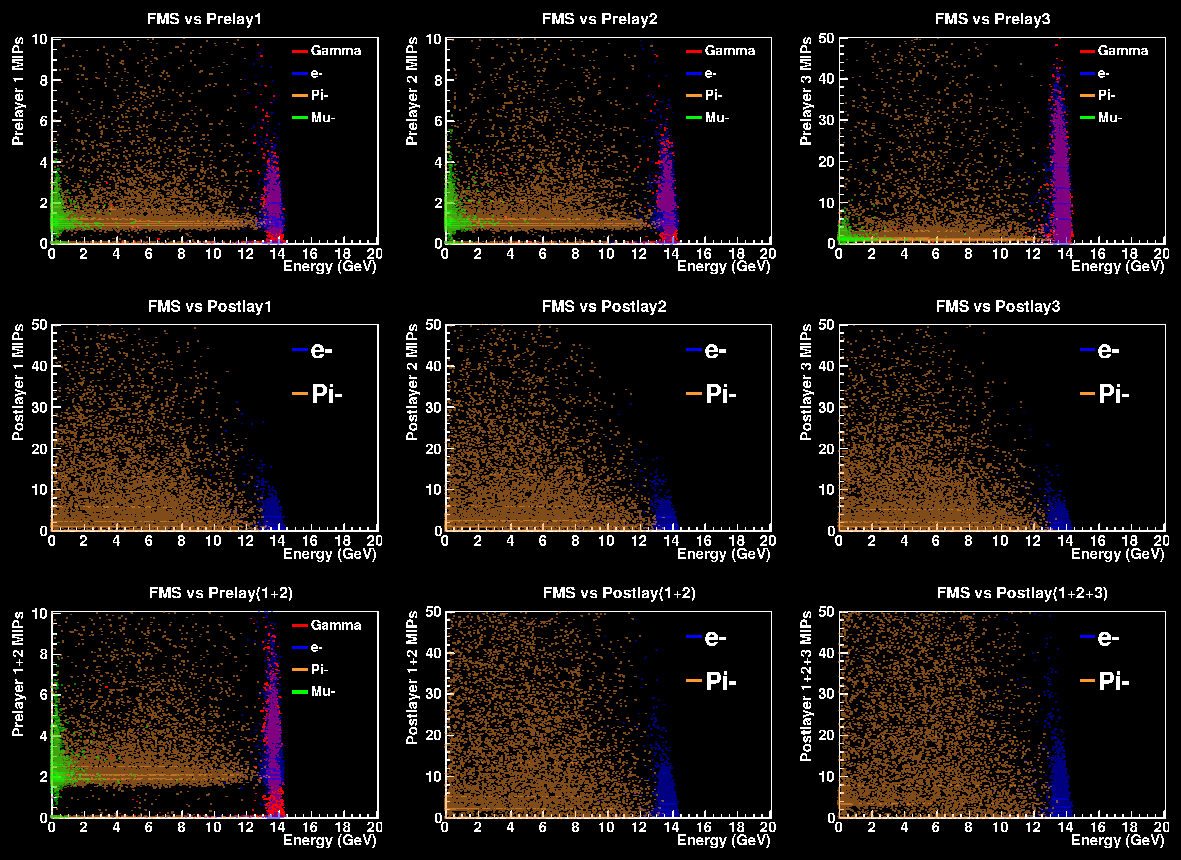
\includegraphics[scale=0.6]{fms_compare_1.ps}}
    }
    \onslide*{2}{
    \rput[lt](0.2cm,0.60cm){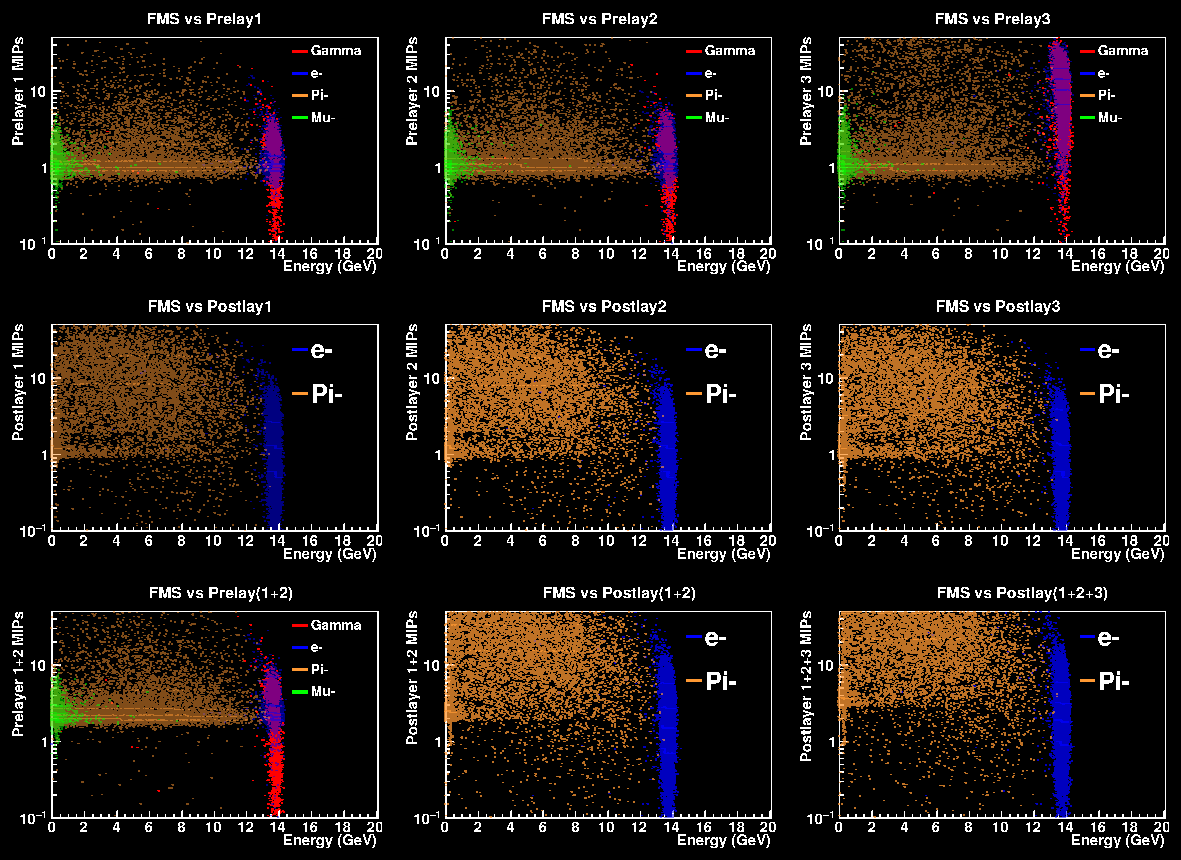
\includegraphics[scale=0.6]{fms_compare_2.ps}}
    }
    \onslide*{3}{
    \rput[lt](0.2cm,0.60cm){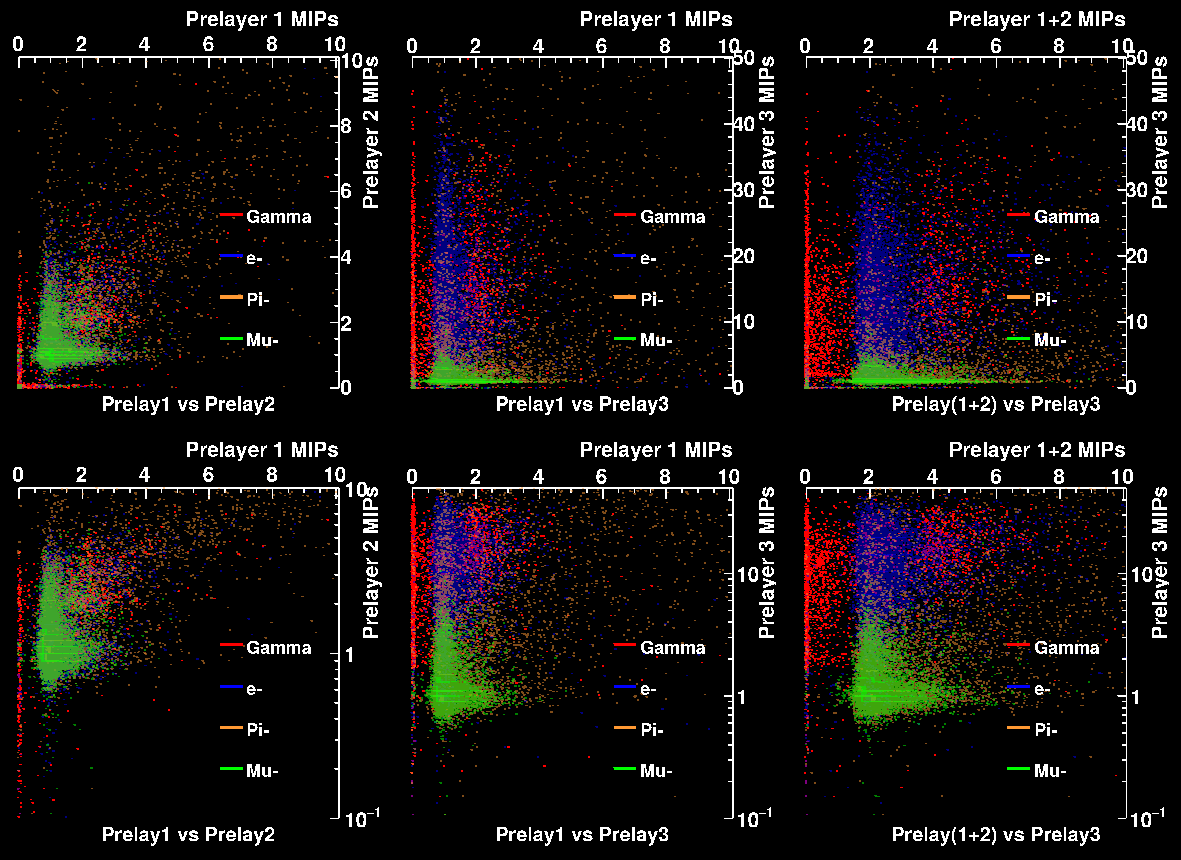
\includegraphics[scale=0.6]{compare_1.ps}}
    }
    \onslide*{4}{
    \rput[lt](0.2cm,0.60cm){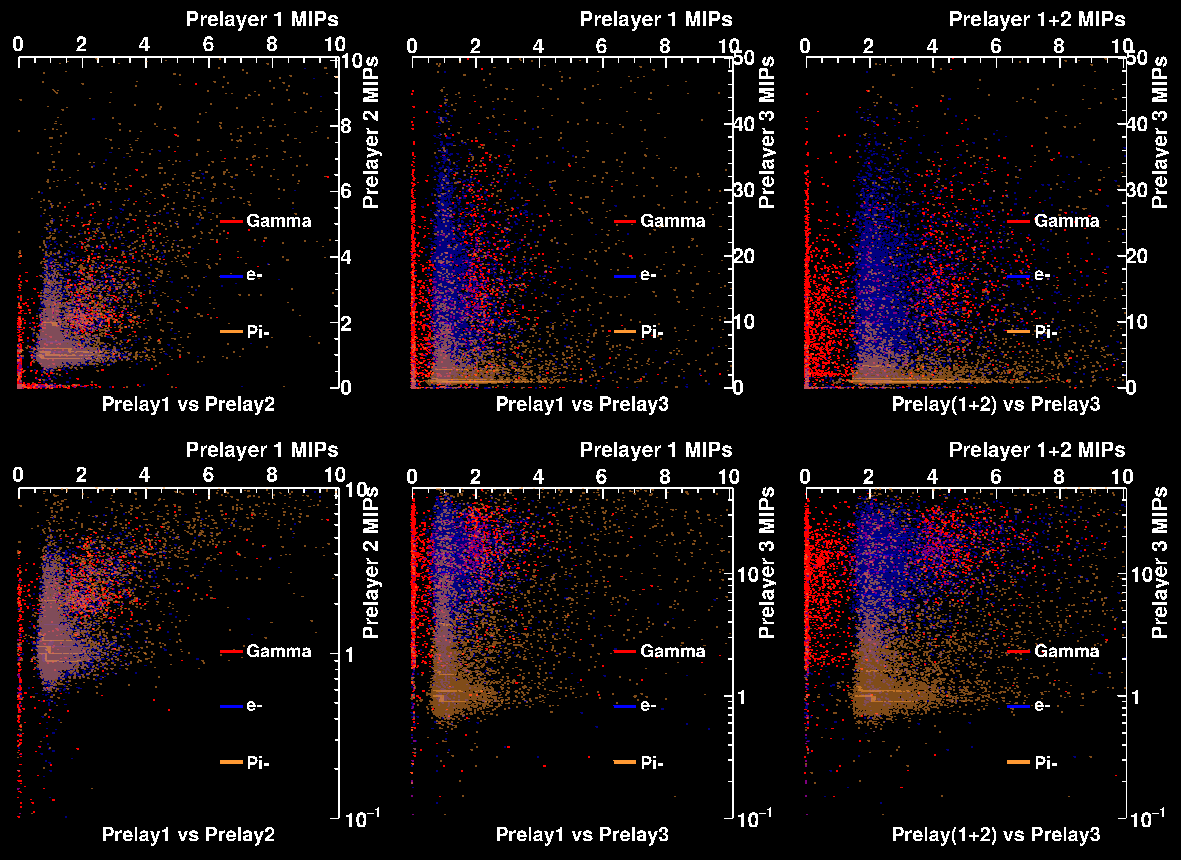
\includegraphics[scale=0.6]{compare_2.ps}}
    }
    \onslide*{5}{
    \rput[lt](0.2cm,0.60cm){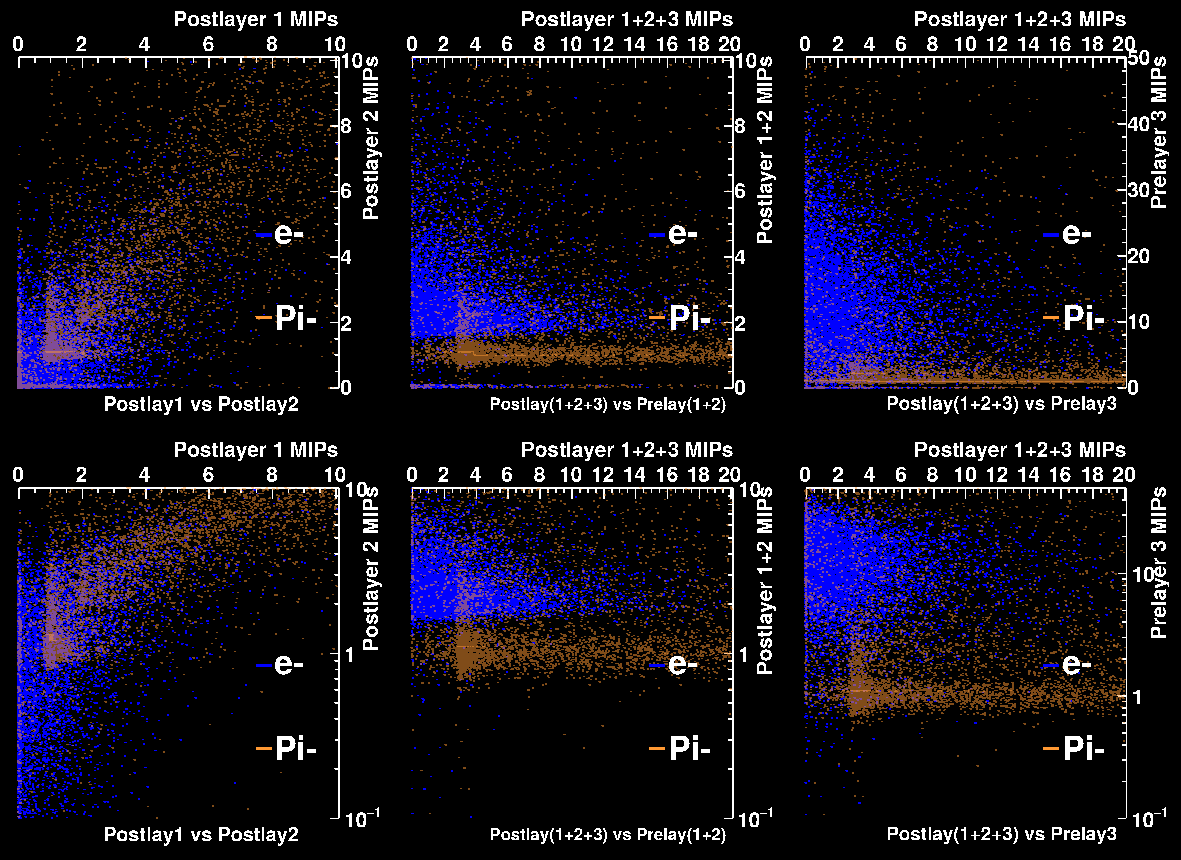
\includegraphics[scale=0.6]{compare_3.ps}}
    }
\end{wideslide}

\end{document}
